\chapter{Materials and Methods}

\section{Materials}

\subsection{Dataset and Structural Priors}
This thesis uses \textbf{AnimeRun}~\cite{animerun} as the core benchmark for both model development and visualization. AnimeRun provides dense optical-flow labels, occlusion cues, and region structure rendered from full-scene animated content in a 2D cartoon style. The dataset is especially suitable for AniUnFlow because it contains the motion patterns that motivate the framework: large stylized displacement, camera-induced parallax, multi-object interaction, and frequent occlusion under flat-color rendering.

In addition to RGB frames, AniUnFlow uses precomputed SAM-style masks as a structural prior. These masks are not treated as motion labels; instead, they define coherent regions that help the framework organize dense matching around objects, parts, and layered boundaries. This distinction is important: the framework remains an \emph{unsupervised optical-flow method}, while segmentation acts only as a structural cue.

To make the dataset characteristics more explicit, Figures~\ref{fig:animerun_dataset_overview} and~\ref{fig:animerun_motion_statistics} summarize the scale and motion profile of AnimeRun as it is used in this thesis. The split-level overview highlights that the benchmark mixes multiple scene families and annotation modalities rather than a single narrow animation template. The motion-statistics view complements this by showing that the dataset contains not only moderate motion pairs, but also a non-trivial tail of higher-displacement cases that are especially relevant for structure-first correspondence reasoning.

\begin{figure*}[t]
    \centering
    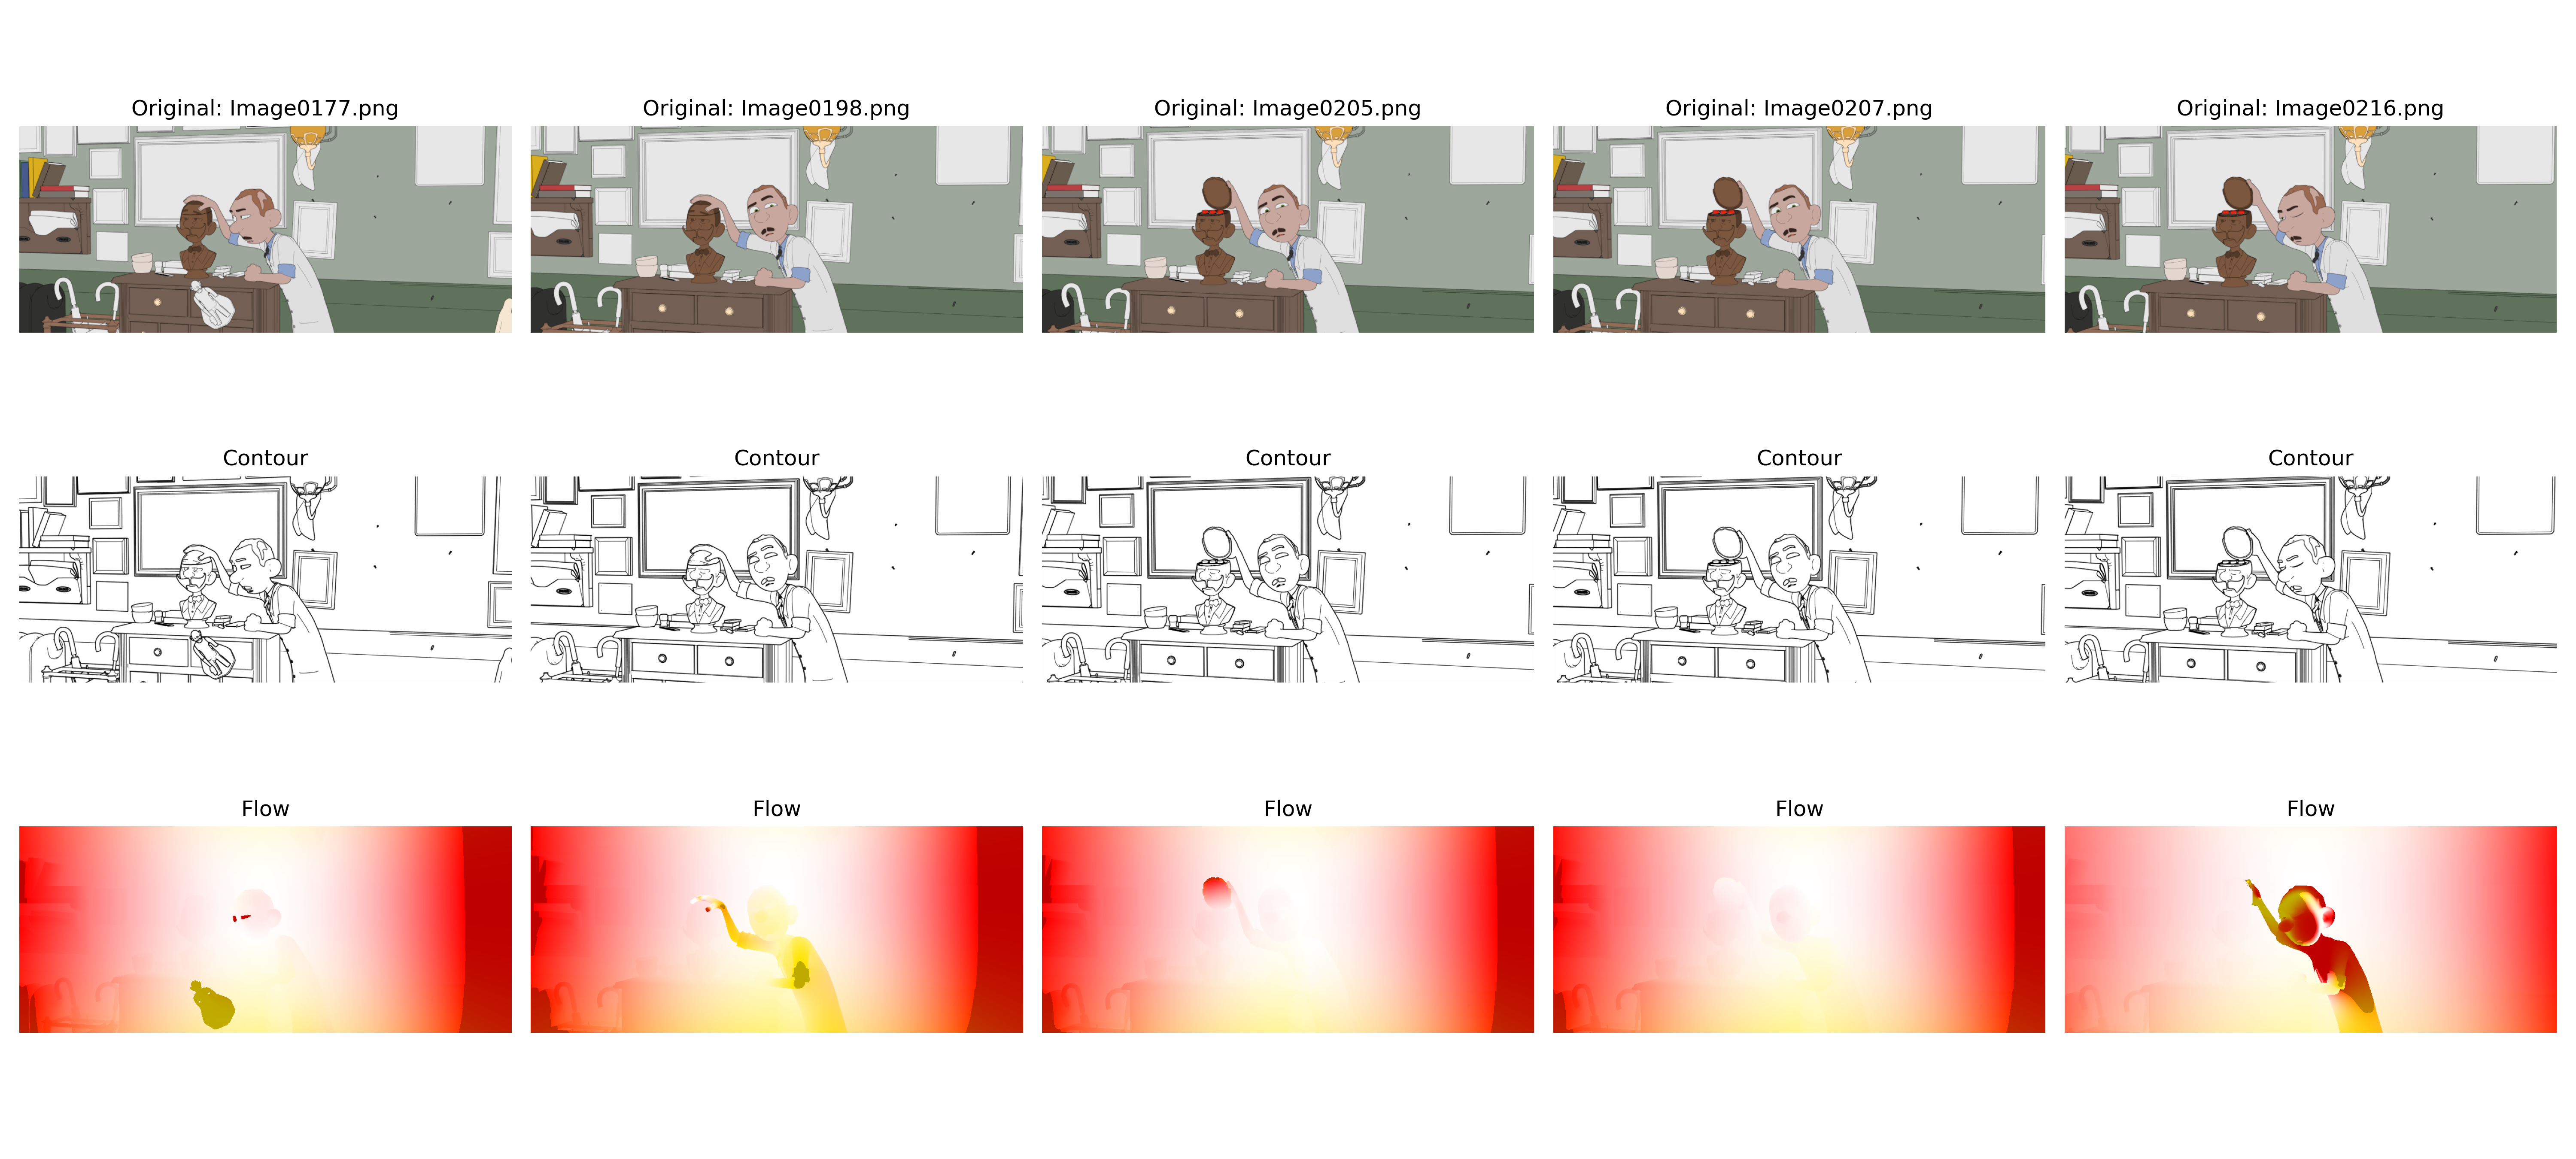
\includegraphics[width=\textwidth]{img/contour_flow_visualization.png}
    \caption{\textbf{Animation-specific correspondence challenges in AnimeRun.}
    Top: representative RGB frames with large flat-color regions. Middle: contour structure that sharply partitions motion boundaries. Bottom: color-coded optical flow showing large stylized displacement. These visual characteristics motivate the structure-first design of AniUnFlow.}
    \label{fig:animerun_contour_flow}
\end{figure*}

\begin{figure*}[t]
    \centering
    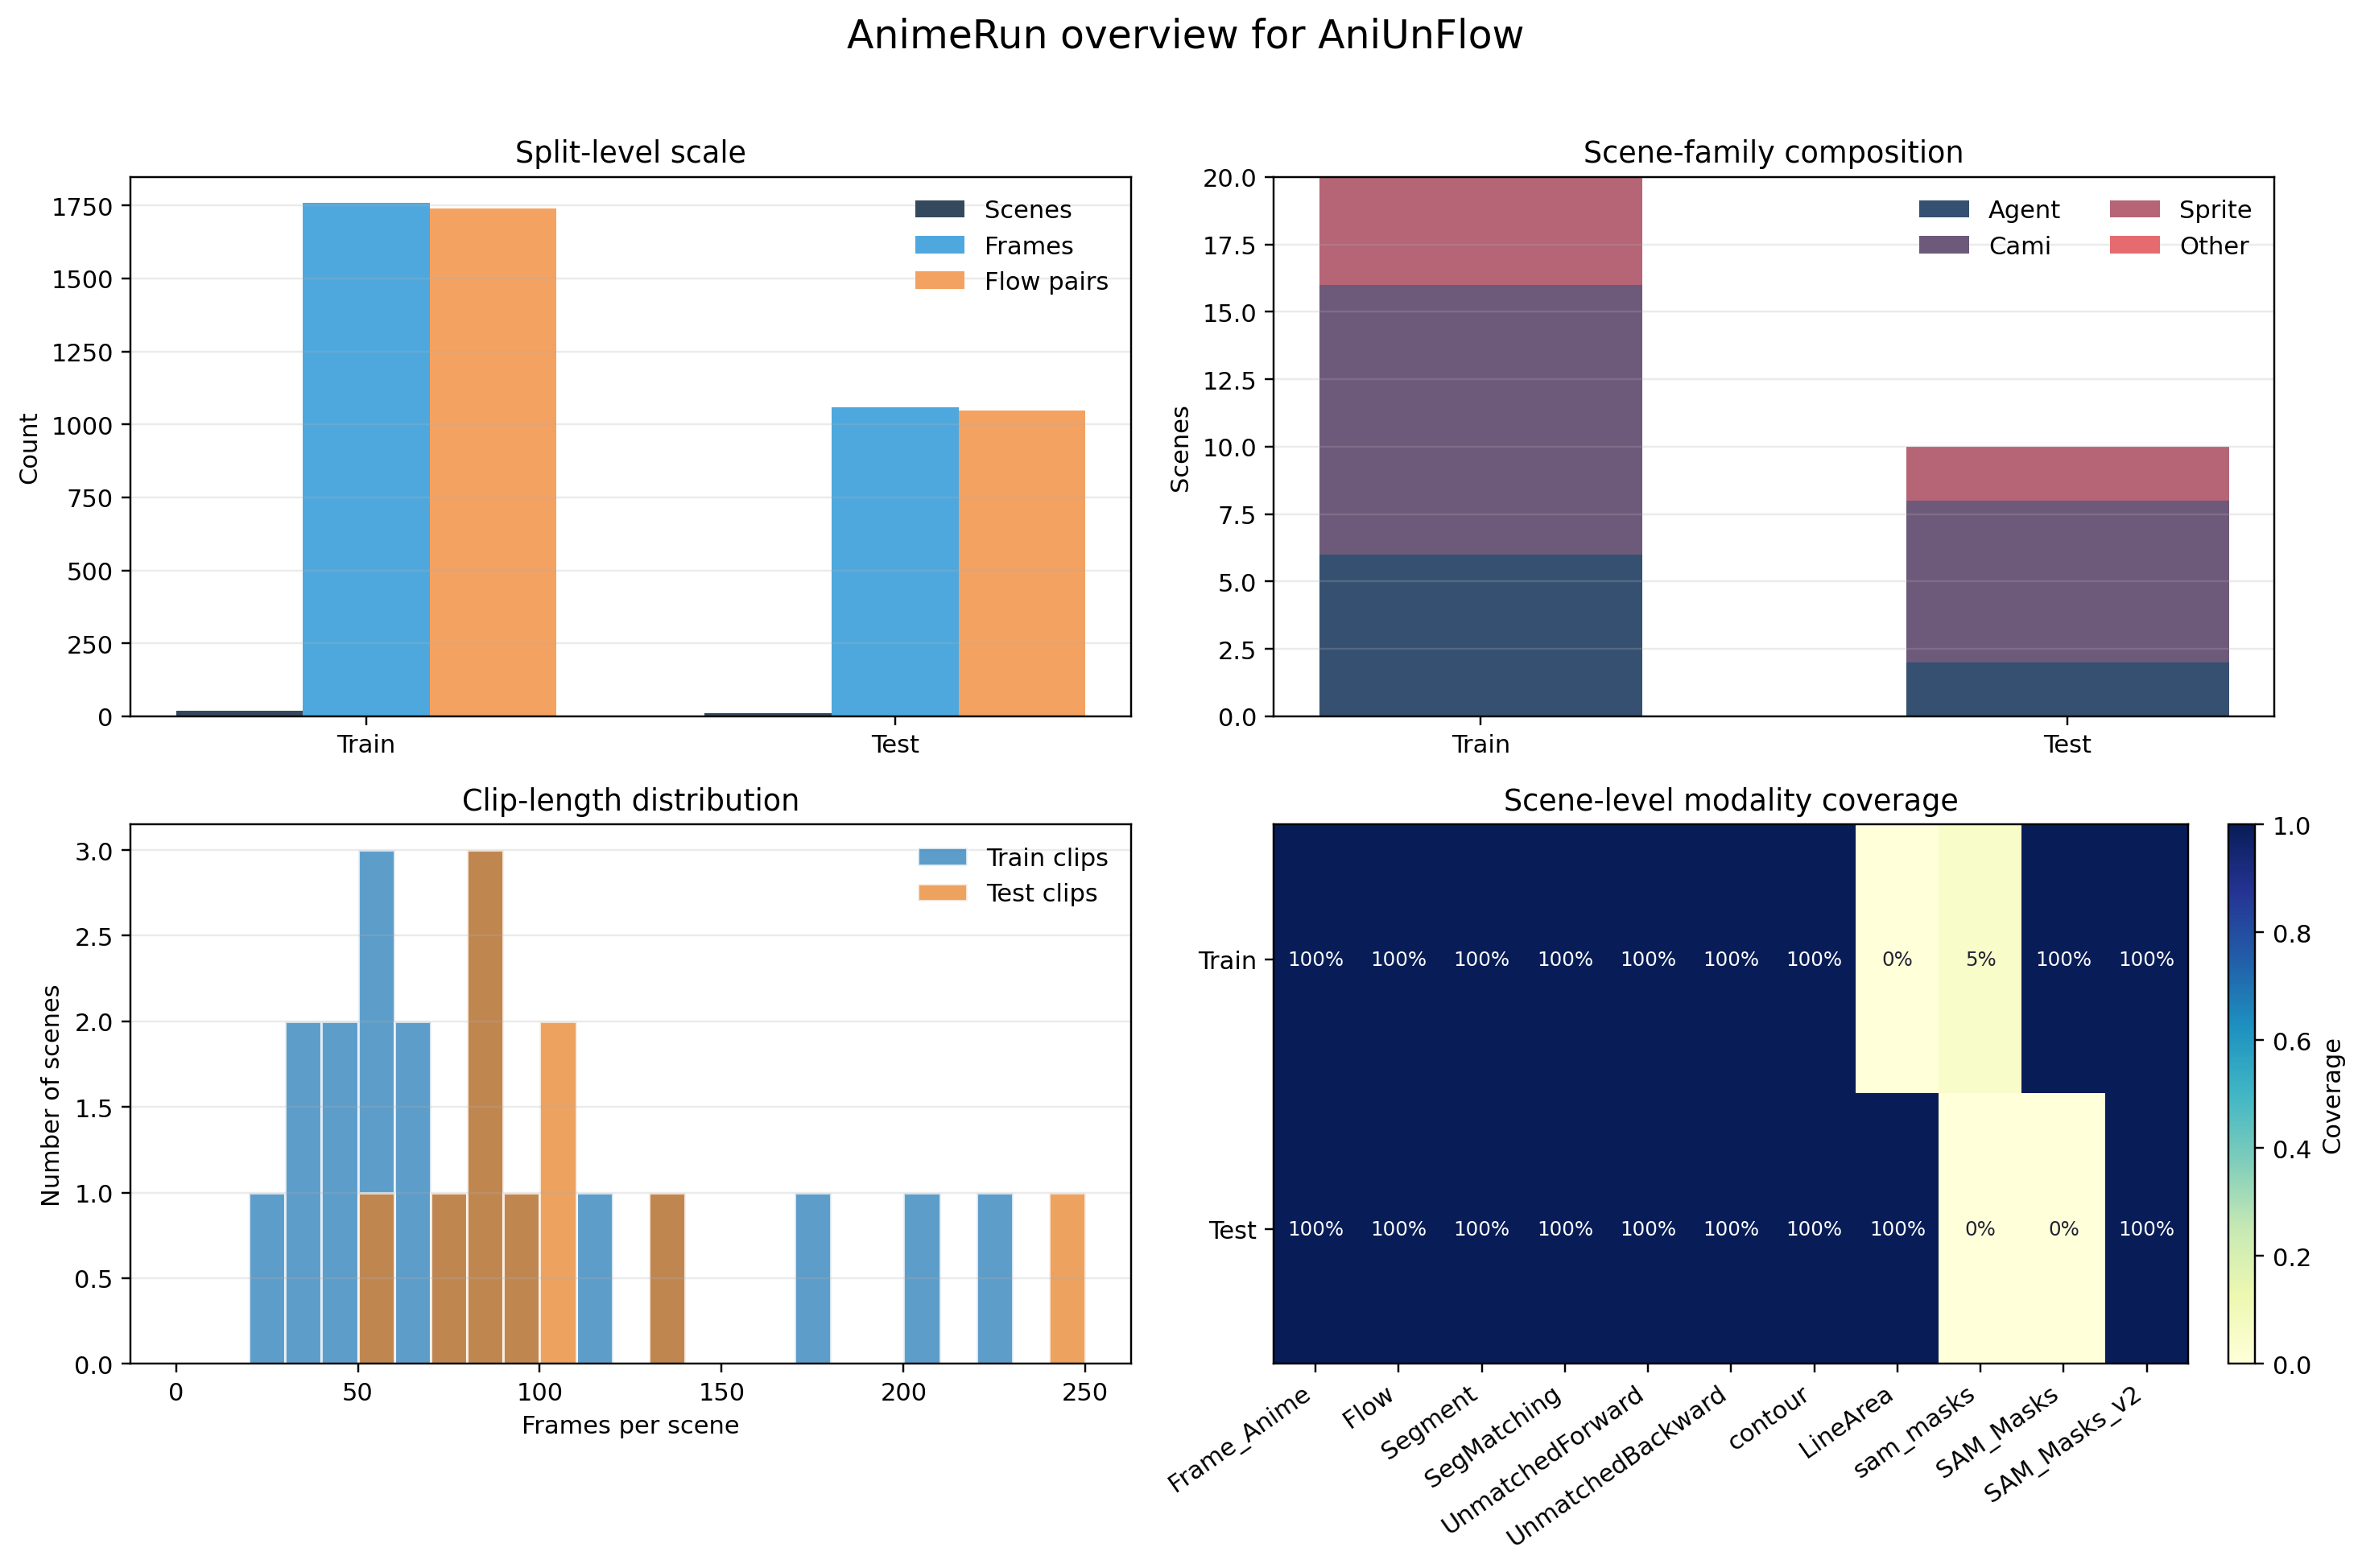
\includegraphics[width=0.92\textwidth]{img/animerun_dataset_overview.png}
    \caption{\textbf{Dataset overview of AnimeRun used by AniUnFlow.}
    The figure summarizes train/test scale, scene-family composition, clip-length distribution, and scene-level annotation coverage. This overview is useful for the thesis because AniUnFlow is trained and analyzed on a benchmark that already couples dense flow, contour structure, segmentation-related assets, and occlusion cues across multiple animation styles and scene layouts.}
    \label{fig:animerun_dataset_overview}
\end{figure*}

\begin{figure*}[t]
    \centering
    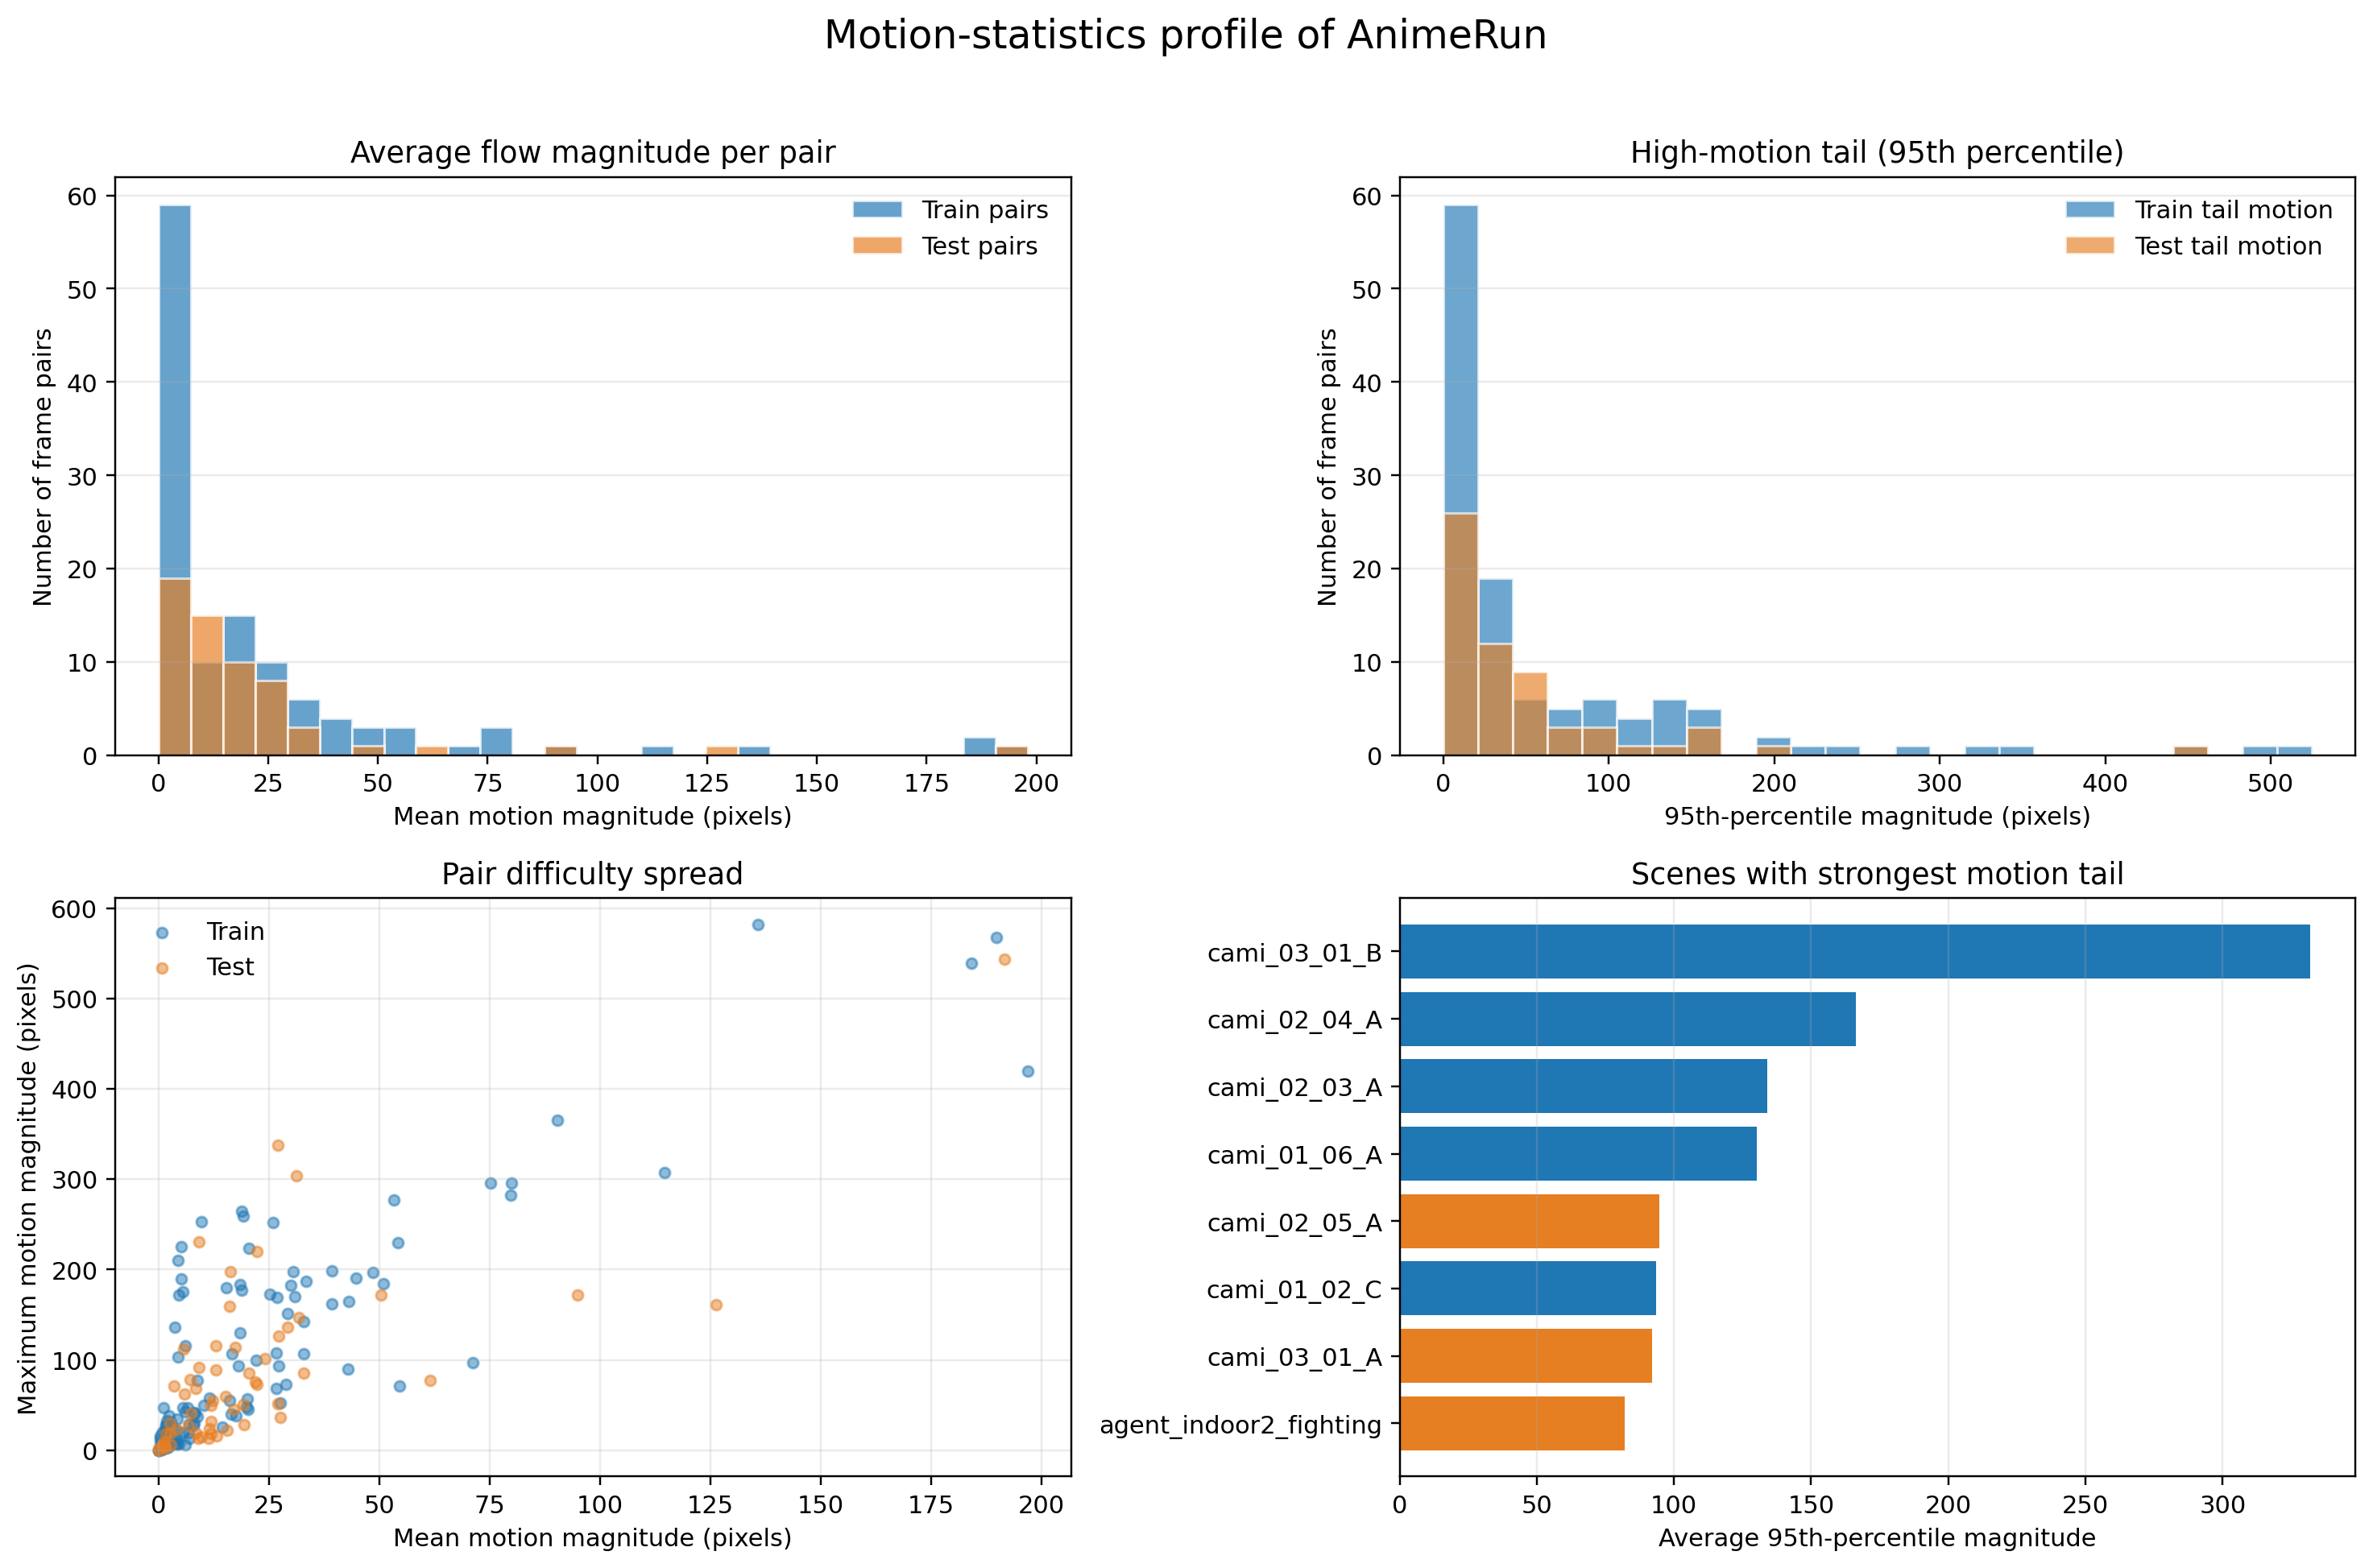
\includegraphics[width=0.92\textwidth]{img/animerun_motion_statistics.png}
    \caption{\textbf{Motion-statistics profile of AnimeRun.}
    Histograms and scatter plots derived from sampled ground-truth flow fields show the distribution of average motion, high-motion tails, pair difficulty, and the hardest scenes in the dataset. The main message is that AnimeRun is not dominated only by easy local motion; it also contains challenging displacement regimes that justify the use of structural priors, temporal memory, and refinement control in AniUnFlow.}
    \label{fig:animerun_motion_statistics}
\end{figure*}

\subsection{Preprocessing and Clip Construction}
Training is performed on short clips rather than isolated frame pairs. Unless otherwise stated, AniUnFlow operates on clips of length $T=5$ and predicts adjacent forward flows $\mathbf{F}_{t\rightarrow t+1}$. Frames are resized and cropped to a fixed training resolution, and all augmentations are applied consistently across the full clip to avoid introducing artificial temporal inconsistency.

We adopt conservative photometric augmentation because strong color jitter can invalidate the weak photometric assumptions already present in stylized animation. Horizontal flips and mild resizing are used when they preserve correspondence structure. SAM masks are cached and resized to match the feature scales used by the framework.

\subsection{Implementation Summary}
AniUnFlow is implemented in PyTorch and trained on AnimeRun with mixed precision, AdamW, gradient clipping, and staged unsupervised optimization. The framework uses a lightweight multi-scale encoder, object-slot pooling from SAM masks, temporal slot memory, dense refinement, and a boundary-aware residual head. The main thesis model uses a conservative multi-stage schedule so that structure-first motion reasoning stabilizes before dense correction becomes dominant.

\section{AniUnFlow Framework}
\label{sec:method}

\subsection{System Overview}

AniUnFlow is designed around a simple principle: \emph{first organize motion estimation by structure, then refine it densely}. Instead of asking a dense matcher to infer everything from scratch, AniUnFlow begins with SAM-guided object regions, compresses them into slot tokens, reasons over those slots temporally, converts them into a structured motion prior, and only then performs dense recovery and residual correction.

\begin{figure*}[t]
\centering
\setlength{\tabcolsep}{4pt}
\renewcommand{\arraystretch}{1.2}
\begin{tabular}{ccccccc}
\fbox{\parbox{0.13\textwidth}{\centering \textbf{SAM}\\structure}} &
$\rightarrow$ &
\fbox{\parbox{0.14\textwidth}{\centering \textbf{Object}\\slot pooling}} &
$\rightarrow$ &
\fbox{\parbox{0.14\textwidth}{\centering \textbf{Temporal}\\slot memory}} &
$\rightarrow$ &
\fbox{\parbox{0.14\textwidth}{\centering \textbf{Structured}\\motion prior}} \\
&&&&&&\\
\fbox{\parbox{0.13\textwidth}{\centering \textbf{Propagated}\\SAM agreement}} &
$\rightarrow$ &
\fbox{\parbox{0.14\textwidth}{\centering \textbf{Dense}\\local refinement}} &
$\rightarrow$ &
\fbox{\parbox{0.14\textwidth}{\centering \textbf{Boundary-aware}\\residual}} &
$\rightarrow$ &
\fbox{\parbox{0.14\textwidth}{\centering \textbf{Final}\\flow field}} \\
\end{tabular}
\caption{\textbf{High-level pipeline of AniUnFlow.} The framework uses object structure to organize the motion hypothesis before dense matching restores local detail. The key thesis-specific addition is the propagated SAM agreement signal, which feeds dense refinement and boundary-sensitive correction.}
\label{fig:aniunflow_pipeline}
\end{figure*}

Given a clip $\mathcal{I}=\{I_t\}_{t=1}^{T}$ and corresponding SAM label maps $\{L_t\}_{t=1}^{T}$, AniUnFlow predicts adjacent dense flow fields without using flow labels during training. The final motion estimate is represented as
\begin{equation}
\mathbf{F}_{t\rightarrow t+1} = \mathbf{F}^{\mathrm{dense}}_{t\rightarrow t+1} + \mathbf{R}_{t\rightarrow t+1},
\end{equation}
where $\mathbf{F}^{\mathrm{dense}}_{t\rightarrow t+1}$ is the refined dense prior and $\mathbf{R}_{t\rightarrow t+1}$ is a boundary-focused residual correction.

\subsection{SAM-Guided Object Representation}

For each frame, AniUnFlow extracts a two-level feature pyramid from the RGB input. Let $\phi_t^{(1)}$ and $\phi_t^{(2)}$ denote the low- and high-level feature maps. The SAM label map is resized to each feature level and used to pool region descriptors into a fixed set of slot tokens:
\begin{equation}
\mathbf{z}_{t,s}^{(l)} = \frac{1}{|\Omega_{t,s}^{(l)}|} \sum_{\mathbf{p} \in \Omega_{t,s}^{(l)}} \mathbf{P}^{(l)}\phi_t^{(l)}(\mathbf{p}),
\end{equation}
where $\Omega_{t,s}^{(l)}$ is the support of slot $s$ at level $l$. The multi-scale pooled descriptors are fused into a single slot representation,
\begin{equation}
\mathbf{z}_{t,s} = f_{\mathrm{slot}}\!\left([\mathbf{z}_{t,s}^{(1)};\mathbf{z}_{t,s}^{(2)}]\right).
\end{equation}

This stage provides two benefits. First, it injects object-level structure into the motion pipeline from the start. Second, it reduces the burden on dense matching by converting flat, ambiguous cartoon regions into compact tokens that are easier to stabilize temporally.

\subsection{Temporal Object Memory and Structured Motion Prior}

Animation correspondence is often unstable when inferred from only two frames because line art flickers, poses deform abruptly, and many regions are locally textureless. AniUnFlow therefore aggregates slot tokens over the full clip with a temporal memory encoder:
\begin{equation}
\widetilde{\mathbf{Z}} = \mathrm{TransformerEnc}(\mathbf{Z} + \mathbf{E}_{\mathrm{time}} + \mathbf{E}_{\mathrm{slot}}),
\end{equation}
where $\mathbf{Z}$ is the stacked slot tensor and $\widetilde{\mathbf{Z}}$ denotes the memory-enhanced slot sequence.

For adjacent frames, AniUnFlow estimates a correspondence matrix between source and target slots using both slot similarity and region overlap priors:
\begin{equation}
\mathbf{A}_t = \mathrm{softmax}\left(\frac{\widetilde{\mathbf{Z}}_t\widetilde{\mathbf{Z}}_{t+1}^{\top}}{\sqrt{D}} + \lambda_{\mathrm{ov}}\mathrm{Overlap}(L_t,L_{t+1})\right).
\end{equation}
The matched slots are then decoded into a structured motion prior. Conceptually, this prior does not need to explain every local deformation perfectly; it only needs to provide a coherent object-centered motion hypothesis that later dense refinement can trust.

\subsection{Propagation-Memory Guidance}

The main structural addition of AniUnFlow is a \emph{propagation-memory} signal built from neighboring SAM masks. The framework warps the previous frame's SAM structure into the current frame using the current motion hypothesis, compares the warped labels to the current SAM labels, and converts their overlap into a dense agreement map:
\begin{equation}
\mathbf{M}_t = g_{\mathrm{agree}}\!\left(\mathrm{warp}(L_{t-1}, \widehat{\mathbf{F}}_{t-1\rightarrow t}),\, L_t\right).
\end{equation}
Here $\widehat{\mathbf{F}}_{t-1\rightarrow t}$ is the available intermediate motion estimate and $\mathbf{M}_t$ is high where propagated structure remains reliable.

\begin{figure*}[t]
\centering
\setlength{\tabcolsep}{4pt}
\renewcommand{\arraystretch}{1.15}
\begin{tabular}{ccccc}
\fbox{\parbox{0.16\textwidth}{\centering Previous\\SAM labels}} &
$\rightarrow$ &
\fbox{\parbox{0.18\textwidth}{\centering Warp by current\\motion hypothesis}} &
$\rightarrow$ &
\fbox{\parbox{0.18\textwidth}{\centering Compare with\\current SAM labels}} \\
&&&&\\
\multicolumn{2}{c}{} &
$\downarrow$ &&
\multicolumn{2}{c}{} \\
&&&&\\
\multicolumn{5}{c}{\fbox{\parbox{0.55\textwidth}{\centering Dense agreement / disagreement map used for confidence modulation, refinement gating, and propagation-memory regularization}}}
\end{tabular}
\caption{\textbf{Propagation-memory mechanism in AniUnFlow.} The framework reuses propagated SAM structure after motion prediction instead of limiting segmentation cues to the front of the pipeline. This dense agreement map is the core visualization-worthy idea that differentiates AniUnFlow from a plain object-memory baseline.}
\label{fig:propagation_memory}
\end{figure*}

The agreement map is used in three places. First, it boosts confidence where propagated structure remains consistent. Second, it raises sensitivity near disagreement regions, which usually correlate with re-association errors, occlusion transitions, or boundary uncertainty. Third, it introduces an explicit propagation-memory regularizer during training so that dense refinement remains compatible with stable structure over time.

\subsection{Dense Refinement and Boundary-Aware Residual}

Once a structured prior is available, AniUnFlow performs dense local refinement at coarse and fine feature levels. Around the current prior $\mathbf{F}^{\mathrm{prior}}$, the framework constructs local correlation volumes,
\begin{equation}
\mathcal{C}_t(\mathbf{p},\Delta) =
\left\langle
\bar{\phi}_{t}(\mathbf{p}),
\bar{\phi}_{t+1}\left(\mathbf{p} + \mathbf{F}^{\mathrm{prior}}(\mathbf{p}) + \Delta\right)
\right\rangle,
\end{equation}
and predicts dense corrections that restore articulated motion, interior deformation, and sharper local geometry.

The dense update is modulated by both slot confidence and propagation-memory confidence:
\begin{equation}
\mathbf{G}_t = \gamma + (1-\gamma)\,c^{\mathrm{slot}}_t \odot c^{\mathrm{dense}}_t \odot \mathbf{M}_t.
\end{equation}
This gate is one of the reasons the framework remains stable: dense matching is encouraged to act aggressively only when object correspondence, local matching, and propagated structure all agree.

After dense refinement, AniUnFlow predicts a final boundary-aware residual
\begin{equation}
\mathbf{R}_{t\rightarrow t+1} =
h\!\left(\phi_t^{(1)}, \phi_{t+1}^{(1)}, \mathbf{F}^{\mathrm{dense}}_{t\rightarrow t+1}, \mathbf{B}_t, \mathbf{Q}_t\right),
\end{equation}
where $\mathbf{B}_t$ is a boundary map derived from SAM masks and $\mathbf{Q}_t$ is a joint confidence signal. The residual branch is intentionally specialized: it concentrates corrective capacity on silhouettes, thin structures, and hard motion transitions rather than relearning the entire flow field.

\subsection{Learning Objective}

AniUnFlow is trained without dense flow supervision. The total objective combines a standard unsupervised flow base with structure-aware regularizers:
\begin{equation}
\mathcal{L} =
\mathcal{L}_{\mathrm{unsup}}
+ \lambda_{\mathrm{sw}}\mathcal{L}_{\mathrm{segwarp}}
+ \lambda_{\mathrm{ds}}\mathcal{L}_{\mathrm{dense\mbox{-}slot}}
+ \lambda_{\mathrm{pm}}\mathcal{L}_{\mathrm{prop}}
+ \lambda_{\mathrm{br}}\mathcal{L}_{\mathrm{boundary}}
+ \lambda_{\mathrm{cyc}}\mathcal{L}_{\mathrm{cycle}}
+ \lambda_{\mathrm{dist}}\mathcal{L}_{\mathrm{distill}}.
\end{equation}

The base term $\mathcal{L}_{\mathrm{unsup}}$ includes photometric reconstruction, smoothness, and forward--backward consistency. Segment-warp consistency keeps the dense prediction compatible with object correspondence. Dense-slot consistency prevents dense refinement from deviating too far from the structured prior inside confident interiors. The propagation-memory term encourages dense predictions to remain aligned with stable propagated structure. Boundary regularization prevents the residual branch from spreading corrective energy uniformly across the whole image. Finally, long-gap cycle constraints and EMA-teacher distillation stabilize learning in later stages.

In practice, the training curriculum is as important as the losses themselves. AniUnFlow begins with a conservative regime in which structure and basic motion alignment stabilize first. Dense correction, long-gap reasoning, and stronger late-stage regularization are enabled only after the object-centered motion hypothesis becomes reliable. This ordering reflects the main philosophy of the framework: dense motion should refine a good structured explanation, not replace it.

\subsection{Representative Visualization of the Framework}

\begin{figure*}[t]
\centering

\includegraphics[width=0.88\textwidth]{img/aniunflow_paper/cami_02_05_A_summary_sheet.png}
\caption{\textbf{Rendered qualitative panels for AniUnFlow.} The figure is generated directly from the framework checkpoint and summarizes three representative clips. Each panel visualizes the full prediction story of the framework, including frame context, predicted motion, and error localization. These rendered examples make the paper substantially more concrete than isolated static crops.}
\label{fig:aniunflow_qualitative_method}
\end{figure*}

Taken together, AniUnFlow follows a coherent and readable progression. SAM-derived structure organizes the scene into motion units, temporal slot memory stabilizes those units over time, propagation memory tells the refiner where temporal structure remains trustworthy, dense matching restores local motion detail, and the final residual branch specializes on the hardest boundary regions. This is the core methodological claim of the thesis: for 2D animation, the most useful optical-flow pipeline is not purely dense and not purely object-level, but a framework in which structure and dense correspondence cooperate at every stage.
